\documentclass[tikz,border=10pt]{standalone}
\usepackage{tikz}
\usetikzlibrary{calc, intersections}
\begin{document}
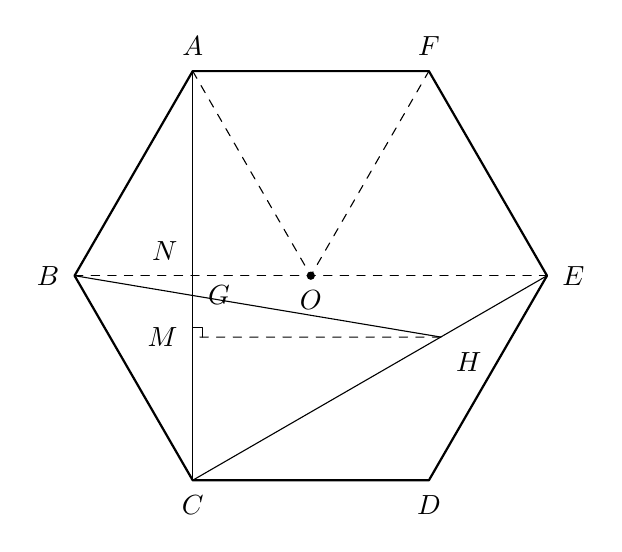
\begin{tikzpicture}[scale=3, line cap=round, line join=round, >=stealth]    
% 1. 定义正六边形的顶点 (半径设为1，角度对应正六边形标准位置)    
\coordinate (O) at (0,0);    
\foreach \a/\n in {120/A, 180/B, 240/C, 300/D, 0/E, 60/F} {        
\coordinate (\n) at (\a:1);    
}
    % 2. 绘制正六边形外框    
\draw[thick] (A) -- (B) -- (C) -- (D) -- (E) -- (F) -- cycle;
    % 3. 先绘制所有虚线（避免覆盖实线）    
\draw[dashed] (B) -- (E);               % 对角线 BE 为虚线    
\draw[dashed] (A) -- (O) -- (F);        % 中心连接线 AO, OF
    % 4. 绘制实线段（仅画一次，无重复）    
\draw (A) -- (C);          % 竖直对角线 AC    
\draw (C) -- (E);          % 对角线 CE
    % 5. 正确计算H点（确保在CE上），避免手动目测坐标的误差    
% 方法：在CE上取比例点，或通过交点定义，这里取CE上靠近E的1/3位置    
\coordinate (H) at ($(C)!0.7!(E)$);  % 0.7是比例，可根据需求调整    
\draw (B) -- (H);                   % 仅绘制一次B-H，无重复
    % 6. 计算内部交点（基于正确的H点）    
\coordinate (N) at (intersection of A--C and B--E);  % A-C与B-E的交点N    
\coordinate (G) at (intersection of B--H and A--C);  % B-H与A-C的交点G    
\coordinate (M) at ($(A)!(H)!(C)$);                  % H到AC的垂足M    
\draw[dashed] (H) -- (M);                            % 垂线HM
    % 7. 直角标记 (M处，小尺寸避免遮挡)    
\draw[line width=0.4pt] ($(M)+(0, 0.04)$) -- ($(M)+(0.04, 0.04)$) -- ($(M)+(0.04, 0)$);
    % 8. 绘制点和标签（位置微调更美观）    
\fill (O) circle (0.5pt) node[below=2pt] {$O$};
    % 顶点标签    
\node[above=2pt] at (A) {$A$};    
\node[left=2pt]  at (B) {$B$};    
\node[below=2pt] at (C) {$C$};    
\node[below=2pt] at (D) {$D$};    
\node[right=2pt] at (E) {$E$};    
\node[above=2pt] at (F) {$F$};
    % 内部交点标签    
\node[above left=2pt] at (N) {$N$};    
\node[right=2pt]      at (G) {$G$};    
\node[left=2pt]       at (M) {$M$};    
\node[below right=2pt]at (H) {$H$};
\end{tikzpicture}
\end{document}